\chapter{Simulating The RV32-Versat Architecture Using The New Verilator Environment}
\label{chapter:sim_verilator}

In this chapter, the new simulation environment for the RV32-Versat architecture
using Verilator is detailed. The Verilator environment was designed to overcome
the disadvantages of typical simulation environments based on the more
traditional event-driven simulators, such as Cadence NCsim and the Synopsys VCS.
As detailed in the previous chapters these simulators are relatively slow,
require expensive licences and complicated the integration of hardware and
software, many times leading to the use of ad hoc solutions.

As explained in Chapter~\ref{chapter:simulators}, event-driven simulators
schedule and process events sequentially, and thus produce more accurate
simulation timing information at the cost of the simulation speed.

In contrast, Verilator is a cycle-accurate simulator and evaluates all logic
elements of the circuit for every clock cycle using binary (0/1) logic. This
produces less accurate results but the simulation is faster. This kind of
simulator does not evaluate any kind of timing in the circuit. However, it can
be used to quickly identify problems at an early stage or after a
change. Additionally, if the architecture is proven in other simulators or in
silicon, Verilator can be used to just capture behaviour modifications.


\section{Working Principle}
\label{section:working_principle}

The simulation environment created for RV32-Versat is based in a set of GNU
Makefiles~\cite{stallman:makefile}. In order to run the simulation environment
the user must go to the root of the RV32-Versat repository and type the command
{\tt make simulator\_name TEST=test\_name}, where the {\tt simulator\_name} is
the name of the desired simulator (Verilator) and {\tt test\_name} is the name
of the folder of the test (driving software program) that must be placed inside
of the folder {\tt tests/test\_name}. The test is compiled, the system memories
are initialized with the program code and data and the system is simulated, following the 
flow shown in Figure~\ref{fig:sim_flow}. This flow will be followed for any program that 
is created and simulated for this architecture.

\begin{figure}[!htb]
	\centering
	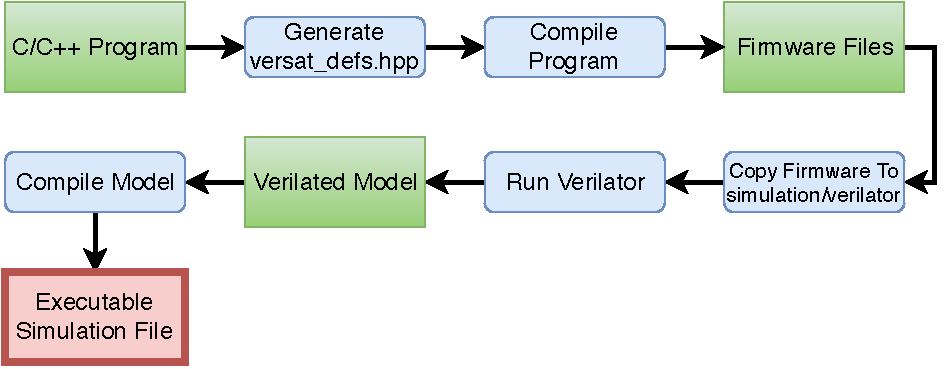
\includegraphics[width=0.95\textwidth]{Figures/Sim_flow.pdf}
	\caption{Simulation flow of the Verilator environment.}
	\label{fig:sim_flow}
\end{figure}

After the {\tt make} command is executed, the Makefile will call another
Makefile placed inside the folder {\tt simulation/verilator} that will then call
another Makefile placed inside the folder {\tt tests/test\_name}. This Makefile
generates the firmware hex files containing the RISC-V program and, if necessary, the 
data to be load into the Versat memories via the testbench, by generating the {\tt 
versat\_defs.hpp} file and compiling the program using the RISC-V toolchain.

The generated firmware files will then be copied into the {\tt simulation/verilator} 
folder where the respective Makefile was called. The next step is to call
Verilator to generate the Verilated model, a C++/System C model obtained from the
synthesizable Verilog files. This model is then linked to the testbench and compiled 
using GNU g++. The resulting executable simulation file will be run and perform 
the actual simulation.

An additional option was added that allows the simulation to be run in machines
that do not have the RISC-V toolchain~\cite{gnu:riscv} installed. This option
compiles the program via SSH in a remote machine where the toolchain is properly
installed. With this option, the user does not need to install the toolchain in
the computer where the simulator is installed, since installing the RISC-V toolchain can 
be a lengthy and complicated process. This option can be activated by adding the flag 
{\tt TOOLCHAIN=FALSE} in the make command.

\section{The Verilator Testbench}
\label{tb_verilator}

The Verilator testbench is considerably different from a typical HDL testbench,
mainly because it is written in C++, SystemC or a compination of both. The use
of these two languages instead of Verilog allows for much greater flexibility by
seamlessly emulating the software of a host system that stimulates the simulated
system. The testbench shown in Figure~\ref{fig:tb_cpp}, written in C++, works
essentially in the same way as the one shown in the previous chapter
(Figure~\ref{fig:tb_verilog}): it loads the hex files to the Versat memories via
the data bus and then runs the program. The simulation finishes when the trap
signal in the PicoRV32 processor is activated, together with an indication that
the program has finished. Optionally, the simulation can output an hex file with
the contents of the Versat memories using the data bus external ports.

\lstset{language=C++}
\begin{figure}[!htb]
	\begin{minipage}{\linewidth}
		\begin{spacing}{0.7}
			\begin{lstlisting}
			#include "Vsystem.h"
			#include "verilated.h"
			#include "verilated_vcd_c.h"
			
			vluint64_t main_time = 0; 
			double sc_time_stamp () {
			return main_time;
			}
			
			int main(int argc, char **argv, char **env)
			{
			Verilated::commandArgs(argc, argv);
			Verilated::traceEverOn(true);
			Vsystem* top = new Vsystem;
			VerilatedVcdC* tfp = new VerilatedVcdC;
			top->trace (tfp, 99);
			tfp->open ("waves.vcd");
			
			top->clk = 0;
			top->databus_sel = 0;
			top->databus_rnw = 1;
			top->databus_addr = 0;
			top->databus_data_in = 1;
			
			int t = 0;
			
			while (!Verilated::gotFinish()) {
			if (t > 200)
			top->resetn = 1;
			top->clk = !top->clk; //Toggle clock
			top->eval();          //Evaluate the model
			tfp->dump (t);        //Write to VCD file
			t += 5;               //Increment clock
			if (top->resetn && top->trap == 1)
			Verilated::gotFinish(true);
			}
			
			tfp->close(); //Close the VCD
			top->final(); //Finish the simulation
			delete top;
			exit(0);
			}
			\end{lstlisting}
		\end{spacing}
	\end{minipage}
	\vspace*{-10mm}
	\caption{Example testbench in C++ for RV32-Versat.}
	\label{fig:tb_cpp}
\end{figure}

The C++ header file created by Verilator from the Verilog model (the Verilated
model) must be included in the C++ testbench. After this, the {\tt
  sc\_time\_stamp} function is invoked, so that the simulator knows the current
time. The simulation setup is done in the {\tt main} function: the runtime
arguments are analysed ( {\tt commandArgs}), the computation of the traced
signals is enabled ( {\tt traceEverOn}), the module to be simulated is declared
( {\tt Vsystem*top}), along with the Verilated VCD model ( {\tt VerilatedVcdC*
  tfp}) and the number of hierarchy levels to be traced are defined ( {\tt
  top->trace (tfp, 99)}). As with the Verilog testbench example, in this example
the data bus external ports are switched off in order to keep the example
simple.

The clock of the circuit is toggled inside the while cycle. For each time that
this cycle executed, the clock signal will be negated, the simulation time will
be checked (to verify if the reset has been disabled), the circuit will be
evaluated ({\tt top->eval()}), the signals will be written to the VCD file ({\tt
  tfp->dump(t)}) and the clock signal time will incremented by 5 ns in each half
period, resulting in a frequency of 100 MHz.The testbench will be executed until
the ( {\tt Verilated::gotFinish}) condition is true. This will happen when the
trap signal is activated and the reset disabled (resetn=1), making the program
leave the while cycle. This will finish the simulation and exit the testbench.

Since the testbench is written in C++/SystemC, it is easy to do software and
hardware co-simulation, given that the host application can be directly embedded
in the testbench. This is a major improvement over other simulation environments
using Verilog testbenches. This is not the only advantage of this new
environment: the simulations using Verilator are considerably faster, as it can
be see in the benchmark presented in the Section~\ref{section:benchmark},
performed for the \ac{CNN} application presented in
Section~\ref{section:application}. Also, since Verilator is a completely free
open-source project, no licence fees are due. This advantages suit perfectly the 
objectives defined for the new simulation environment.
The major disadvantage of this new simulation environment is its lower
precision when compared with environments using event-driven simulators. This
happens because Verilator does not provide timing information, since it does not
take into account propagation times and because Verilator uses a 2-state model,
assuming that all the signals in a circuit have a value that can either be 0 or
1.  However, this disadvantage is many times irrelevant in the context of the
RV32-Versat architecture, since this architecture has already been extensively
tested in \ac{FPGA}s and with other simulators.

%%%%%%%%%%%%%%%%%%%%%%%%%%%%%%%%%%%%%%%%%%%%%%%%%%%%%%%%%%%%%%%%%%%%%%%%
